%%%%%%%%%%%%%%%%%%%%%%%%%%%%%%%%%%%%%%%%%%%%

% formato FRONTE RETRO
\documentclass[epsfig,a4paper,11pt,titlepage,twoside,openany]{book}
\usepackage{epsfig}
\usepackage{plain}
\usepackage{setspace}
\usepackage[paperheight=29.7cm,paperwidth=21cm,outer=1.5cm,inner=2.5cm,top=2cm,bottom=2cm]{geometry} % per definizione layout
\usepackage{titlesec} % per formato custom dei titoli dei capitoli

\singlespacing

\usepackage[italian]{babel}

%%%%%%%%%%%%%%%%% STEFANO ADDED %%%%%%%%%%%%%%%%
% supporto lettere accentate
% queste due righe nel preambolo servono a poter utilizzare le lettere accentate in tutto il testo se no di norma si inserirebbero con \'e...
\usepackage[T1]{fontenc}
\usepackage[utf8]{inputenc}
\usepackage{hyperref} %Serve per i riferimenti
\usepackage{caption}  %Serve per le note (caption)
\usepackage{multicol}	 %Serve per usare più colonne

%%%%%%%%%%%%%%%%% ENRICO ADDED %%%%%%%%%%%%%%%%%
\usepackage{ulem} %Serve per il sottolineato
\usepackage{amsmath} %Serve per alcuni ambienti matematici
\usepackage{array} %Serve per le tabelle
\usepackage{multirow} %Seve per tabelle
\setcounter{secnumdepth}{5} %Utilissimo serve per aumentare il numero di paragrafi, si arriva fino a 5 livelli di profondità x.x.x.x.x
%GRAFICI
\usepackage{pgfplots}
\usepackage{pgfmath}
\usepackage{tikz}
%CODICE
% \usepackage{listings}
% \usepackage[cache=false]{minted} 
%\setminted{tabsize=4, breaklines, breakanywhere, linenos, mathescape,}

% \lstset{
% 	  breakatwhitespace=false,         
% 	  breaklines=true,     
% 	  basicstyle=\footnotesize\ttfamily,            
% 	  commentstyle=\color{blue}, %Indica il colore dei commenti
% 	  keywordstyle=\color{red}, %Indica il colore delle parole chiave
% 	  language=C, %Indica il linguaggio predefinito da usare
% 	  rulecolor=\color{black}, %Indica il colore dei numeri di righe
% 	  tabsize=4,
% 	  escapeinside={\%*}{*)},
% 	  morekeywords={}, %Altre parole da inserire tra le keywords. Ad esempio possiamo aggiungere do, gotttto, ecc ecc 
% }
%%%%%%%%%%%%%%%%% END OF ENRICO  %%%%%%%%%%%%%%%%

\begin{document}
%set the language of the text to italian
% !TeX spellcheck = it_IT

%%%%%%% personal commands (ALIAS):
% \newcommand{\nome_commando}[argomenti]{comando}
\newcommand{\e}[1]{$\cdot 10^{#1}$}
\newcommand{\mmax}[0]{mod\_withMax }
\newcommand{\mover}[0]{mod\_overlap }
\newcommand{\mmod}[0]{modularità modificata }
\newcommand{\nv}[0]{Node2Vec }
\newcommand{\wv}[0]{Word2Vec }
\newcommand{\cnrl}[0]{CNRL }
\newcommand{\cora}[0]{Cora }
\newcommand{\citeseer}[0]{Citeseer }
\newcommand{\LPred}[0]{Link Prediction }
%



%
\chapter{Esperimenti}\label{chap:3}
In questo capitolo vi è una raccolta rappresentativa degli esperimenti svolti, con le relative analisi e commenti.
\section{Origini dei grafi}
In questa sezione vengono spiegati i dataset utilizzati e cosa rappresentano.\\
Si possono dividere in due gruppi. Perché presentano caratteristiche d'affinità, inoltre i grafi dei due gruppi sono stati utilizzati nel corso del tirocinio per applicazioni differenti.\\
Nella Tabella~\ref{tab:dati_grafi} sono elencati i dettagli tecnici di ogni dataset.
%
\begin{center}
	\begin{tabular}{|l|r|r|r|c|c|r|}
		\hline
		nome&nodi&archi&archi/nodi&diretto&etichette&attributi\\
		\hline
		\cora & 2708 & 5429 & 2.0 & sì & 7 & 1433\\
		\citeseer & 3312 & 4732 & 1.4 & sì & 6 & 3703\\
		\hline
		BlogCatalog & 10312 & 333983 & 32.4 & no & 39 & 0\\
		Gnutella & 6301 & 20777 & 3.3 & no & 0 & 0\\
		Dolphins & 62 & 159 & 2.6 & no & 0 & 0\\
		Karate & 35 & 78 & 2.2 & no & 0 & 0\\
		\hline
		\end{tabular}
		\captionof{table}{Per ogni grafo sono indicate le sue caratteristiche principali}
		\label{tab:dati_grafi}
\end{center}
%
\subsection*{Esperimento principale: \cora\ - \citeseer}\cite{Co-Ci_1}\cite{Co-Ci_2}
Il dataset \textbf{\cora} è un grafo diretto che rappresenta una rete di articoli scientifici sull'apprendimento automatico. Ogni nodo è un articolo, mentre ogni arco rappresenta il collegamento fra un documento e l'altro; se il documento $A$ cita il documento $B$, si avrà l'arco $(A, B)$. La rete è costruita in modo che ogni nodo abbia almeno un arco entrante o uscente.\\
Ogni articolo appartiene esattamente ad una classe identificata da un etichetta. Ogni attributo rappresenta la presenza o meno di una determinata parola nel testo del documento (deve apparire almeno 10 volte).\\
\\
Il dataset di \textbf{\citeseer} è un grafo diretto che rappresenta una rete analoga a quella di \cora; anche in questo caso si hanno articoli scientifici che si citano vicendevolmente. L'etichetta è la classe d'appartenenza di cui l'articolo fa parte, e gli attributi rappresentano nuovamente la presenza o meno di certe parole all'interno del testo.\\
%
\subsection*{Grafi per esperimenti minori}
Questi quattro grafi vengono presentati in ordine decrescente nel numero dei nodi, così come fatto nella seconda parte della Tabella~\ref{tab:dati_grafi}.\\
\begin{itemize}
	\item \textbf{BlogCatalog}\cite{BlogCatalog} rappresenta la rete di relazioni, di conoscenza, fra gli utenti di alcune piattaforme per blog
	\item \textbf{Gnutella}\cite{Gnutella_1}\cite{Gnutella_2} descrive la rete peer-to-peer per lo scambio di file di Gnutella nell'agosto 2002. Ogni nodo rappresenta un host e ogni arco un collegamento fra due host
	\item \textbf{Soc-Dolphins}\cite{Dolphins_1}\cite{Dolphins_2} riporta la rete sociale di un gruppo di delfini al largo della Nuova Zelanda nel 2003
	\item \textbf{Karate}\cite{Karate} raccoglie lo storico degli incontri in un club di karate universitario nel 1977. Ogni nodo è un membro del club, ogni arco indica uno scontro terminato in pareggio.
\end{itemize}
%
\section{Modello di un grafo}
In questa sezione viene spiegato cosa si intende per modello di un grafo, e perché è tanto importante per gli algoritmi che vi sono costruiti sopra.\\
Come descritto nel capitolo sull'implementazione è necessario visitare il grafo per generare su questo dei cammini. Tali vettori di nodi vengono presi in input dall'algoritmo di \wv\ che, tramite una rete neurale va a descrivere ogni nodo coinvolto tramite un vettore di valori reali. \cnrl\ utilizza invece un metodo alternativo chiamato Latent Dirichlet Allocation (LDA)\cite{LDA} o una sua variante detta HalfLDA, entrambe sono comunque basate su \wv.\\
\begin{figure}[htp]
	\centering
	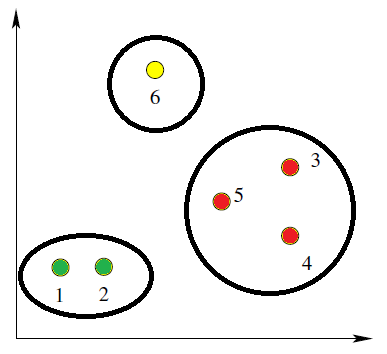
\includegraphics{immagini/punti_modello}
	\caption{Sono visualizzati i nodi di un grafo rappresentati da un modello che dispone di due dimensioni, mostrato in Tabella~\ref{tab:coordinate_modello}}
	\label{fig:grafico_modello}
\end{figure}
\\
\begin{center}
	\begin{tabular}{|l|cc|}
		\hline
		ID&X1&X2 \\
		\hline
		1 & 1 & 2 \\
		2 & 2 & 2 \\
		3 & 7 & 5 \\
		4 & 7 & 3 \\
		5 & 5 & 4 \\
		6 & 3 & 8 \\
		%7 & 1 & 5 \\
		%8 & 1 & 7 \\
		%9 & 1 & 8 \\
		\hline
	\end{tabular}
	\captionof{table}{Tabella rappresentativa del modello dei nodi in Figura~\ref{fig:grafico_modello}}
	\label{tab:coordinate_modello}
\end{center}
%\begin{center}
%	\begin{tabular}{|l|ccccccccc|}
%		\hline
%		ID & 1 & 2 & 3 & 4 & 5 & 6 & 7 & 8 & 9 \\
%		\hline
%		X1 & 1 & 2 & 7 & 7 & 5 & 3 & 1 & 1 & 1 \\
%		X2 & 2 & 2 & 5 & 3 & 4 & 8 & 5 & 7 & 8 \\
%		\hline
%	\end{tabular}
%	\captionof{table}{Tabella rappresentativa del modello dei nodi in Figura~%\ref{fig:grafico_modello}}
%	\label{tab:coordinate_modello}
%\end{center}
Di norma ogni vettore contiene $64$ numeri reali, ognuno dei quali rappresenta una posizione lungo un asse in uno spazio a $64$ dimensioni. È possibile pensare anche ad un caso più semplice. In Figura~\ref{fig:grafico_modello} si possono vedere sei punti che si può immaginare appartenessero ad un grafo e fossero legati fra loro in qualche modo. Una volta generati i cammini su tale grafo, e questi forniti ad uno dei due algoritmi, viene calcolata la Tabella~\ref{tab:coordinate_modello}. Ad ogni ID di un nodo vengono associati due valori (qui interi per semplicità). Se ne usano due in quanto facili da mostrare, con $64$ sarebbe pressoché impossibile. Si possono dunque immaginare come coordinate su un piano cartesiano, e così si arriva alla Figura~\ref{fig:grafico_modello}, visivamente si può dire che esistono 3 gruppi distinti evidenziati dai colori, abbiamo quindi $(1, 2) - (3, 4, 5) - (6)$.\\
Escludendo l'influenza causata dai colori, il nostro occhio ci suggerisce l'esistenza di questi 3 gruppi in quanto i nodi che vi fanno parte sono vicini fra loro. Questo ricalca alla perfezione la definizione di somiglianza: tanto più due nodi sono vicini tanto più questi sono simili. Si ricorda che esistono comunque molte definizioni formali di somiglianza e la distanza euclidea è solo una di queste.\\
\\
Se due nodi molto simili, e quindi vicini, vengono collegati da un arco, allora tale arco assume un valore molto elevato, vicino a $1$, diversamente assumerà un valore molto basso, vicino a $0$, se i nodi che lega sono diversi ossia molto lontani.\\
Questo valore verrà chiamato d'ora in avanti coerenza di un arco\footnote{Non esiste un vero e proprio termine tecnico per questa definizione}.
%
\section{Link Prediction}
Questo è il primo di tre algoritmi, che verranno illustrati in questo capitolo, tutti e tre basati sul modello del grafo appena spiegato.\\
L'algoritmo di \LPred\ ha lo scopo d'assegnare un valore al grafo in input. Questo valore è una percentuale e per tale motivo ricade nell'intervallo $[0, 1]$. Questa percentuale sta a rappresentare la coerenza degli archi del grafo. Nel dettaglio, un arco è molto coerente se lega due nodi simili; un grafo è tanto più coerente quanti più archi coerenti ha.
%
\subsection{Dinamiche di funzionamento}
In prima istanza viene caricato il grafo, sempre come lista d'archi, sono questi il fulcro dell'algoritmo. Si va poi a spezzare gli archi in due gruppi, dopo averli mescolati per non creare delle divisioni sempre uguali. Tale separazione viene fatta sulla base del parametro $F$, che indica quale sarà la percentuale degli archi adibiti all'addestramento del modello e quali invece saranno adibiti alla fase di test.\\
Il numero degli archi usati per il test viene dato dalla Formula~\ref{eq:n_archi_fake}
\begin{equation}
	m \cdot \frac{1}{F}
	\label{eq:n_archi_fake}
\end{equation} 
\begin{equation}
	m \cdot \left( 1- \frac{1}{F} \right)
	\label{eq:n_archi_true}
\end{equation}
mentre quelli utilizzati per l'addestramento corrispondono alla Formula~\ref{eq:n_archi_true}, dove $m$ è il numero di archi del grafo.\\
Il nuovo grafo (\textbf{G1}) creatosi, inseguito alla rimozione degli archi per il test, viene utilizzato per generare il modello.\\
Per ogni arco appartenente all'insieme di test (\textbf{Test=T}) se ne genera un altro (\textbf{Check=C}) tramite una coppia di nodi casuali, assicurandosi che non corrispondano ad un arco già esistente. Si hanno quindi tre insiemi, il primo adibito all'addestramento, stabilisce il modello necessario a discernere quale delle due restanti selezioni è la migliore.
Per ogni arco, di T e di C, si va a vedere quanto sono simili i nodi che legano e se ne calcola così la coerenza, tramite l'apposita funzione di similarità, ora disponibile. Gli archi possono essere valutati sulla base di questo nuovo parametro.\\
Si è interessati a capire quanto sono buoni gli archi originari del grafo (T), rispetto a quelli generati casualmente (C). 
\begin{equation}
	\frac{\left( n_1 + \frac{n_2}{2} \right)}{n}
	\label{eq:AUC_formula}
\end{equation}
Si usa perciò la metrica detta \textbf{AUC}\cite{AUC_metric}, che si basa sulla Formula~\ref{eq:AUC_formula}, i cui elementi sono:
\begin{itemize}
	\item $n$ è il numero di archi presenti nell'insieme di test, calcolato mediante la Formula~\ref{eq:n_archi_fake}
	\item $n_1$ sono le volte in cui un arco di test T è migliore di un arco casuale di C
	\item $n_2$ sono le volte in cui un arco di test T ha valore pari o quasi rispetto ad un arco casuale di C
\end{itemize}
Per ogni arco di T se ne associa casualmente un altro di C. Si guarda quanto valgono i due archi coinvolti. Se l'arco di T vale più dell'arco di C si incrementa di $1$ il valore di AUC, se uguali o quasi (differenza inferiore ad una soglia detta $ \epsilon$) si incrementa di $0.5$. Avendo fatto ciò con ogni arco se ne calcola la media.\\
\\
Il valore finale della metrica AUC dipende fortemente da quale metodo si adotta per abbinare gli archi appartenenti a T e C. Un accoppiamento sbagliato può fortemente sbilanciare il risultato, è per questo motivo che si va ad utilizzare un abbinamento casuale.\\
Il parametro $F$ influisce sul risultato finale. Più questo si avvicina a $1$ più cresce il numero di archi da utilizzare per la selezione di test, di conseguenza diminuiscono i dati su cui fare affidamento per creare un buon modello che rappresenti appieno il grafo di partenza. Il valore finale da aspettarsi è quindi tendenzialmente più basso.\\
È necessario ricordare che la stima qui calcolata dipende fortemente dalla selezione iniziale. È per questo motivo che tutto il processo non viene svolto solo una volta bensì $F$ volte, così da andare a stabilizzare il valore calcolato tramite la media di tutte le iterazioni. Inoltre questo permette di utilizzare via via tutti gli archi per addestrare il modello di \textbf{G1}.\\
\\
L'intero algoritmo si basa sul confronto degli archi grazie al valore che li rappresenta, per individuare i più rilevanti. La parte critica è la generazione di tale valore mediante la funzione di similarità.\\
Tale funzione può essere definita in svariate maniere in quanto si possono pesare diversi aspetti. Un esempio classico è basato sulla distanza euclidea: più due nodi sono distanti nella rappresentazione del modello meno sono simili. Verranno mostrate le applicazioni di altre funzioni di similarità basate su diversi principi che però non verranno qui riportati.
%
\subsection{Esempio}
\begin{center}
	\begin{tabular}{|c|c|c|c|}
		\hline
		arco & autentico & dist & AUC\\
		\hline
		3-4 & sì & $2$ & \multirow{2}{*}{$1$}\\
		2-6 & no & $\sqrt{37}$ & \\
		\hline
		4-5 & sì & $\sqrt{5}$ & \multirow{2}{*}{$0.5$}\\
		3-5 & no & $\sqrt{5}$ & \\
		\hline
		5-6 & sì & $\sqrt{20}$ & \multirow{2}{*}{$0$}\\
		2-5 & no & $\sqrt{13}$ & \\
		\hline
		1-2 & sì & $1$ & \multirow{2}{*}{$1$}\\
		1-3 & no & $\sqrt{45}$ & \\
		\hline
	\end{tabular}
	\captionof{table}{Tabella riassuntiva del procedimento di \LPred}
	\label{tab:dati_es_prediction}
\end{center}
Si consideri il modello descritto tramite la Figura~\ref{fig:grafico_modello} e la Tabella~\ref{tab:coordinate_modello}. Si sa inoltre che $F=2$, gli archi originali adibiti al test sono $(1, 2), (3, 4), (4, 5), (5, 6)$ mentre quelli generati casualmente sono $(3, 5), (2, 5), (2, 6), (1, 3)$. I due insiemi sono nello stesso numero per creazione e per essere facilmente confrontati.\\
Nelle prime due colonne della Tabella~\ref{tab:dati_es_prediction} sono riassunti gli archi e la loro origine. Le colonne seguenti rappresentano invece i passaggi successivi dell'algoritmo.\\
Nella terza colonna si può notare che ad ogni arco è stato associato un valore rappresentativo della distanza euclidea misurata sul piano cartesiano fra i due estremi dell'arco. La funzione di similarità premia i valori più bassi a discapito degli altri. Inoltre la Tabella è stata ordinata in modo che tutti gli archi di un insieme siano associati con uno dell'altro in maniera casuale. Si può notare che nella seconda colonna "sì" e "no" s'alternano.\\
Nell'ultima colonna viene rappresentato l'incremento che si andrà ad apportare alla metrica AUC grazie alla valutazione dei due archi corrispondenti. Questo valore dovrà poi esser diviso per il numero delle coppie in gioco per riportarlo nell'intervallo $[0, 1]$, in questo caso risulta $ \frac{\left( 1+0.5+0+1 \right)}{4} = 0.625$.\\
Si possono osservare alcune peculiarità:
\begin{itemize}
	\item l'accoppiamento degli archi viene fatto in maniera casuale per evitare uno sbilanciamento
	\item nel caso mostrato una selezione a favore degli archi autentici porterebbe ad avere un incremento nullo del valore di AUC, al contrario si potrebbe avere un incremento di due unità se si favorissero  gli archi generati casualmente
	\item non si hanno archi ripetuti perché viene impedito durante la creazione, ma questo non vuol dire che un arco di C non possa corrispondere ad un arco usato in principio per generare il modello
	\item si può immaginare che più il valore di $F$ è grande e quindi più è grande la selezione di archi per l'addestramento (grazie alla Formula~\ref{eq:n_archi_true}), più il valore di AUC calcolato cresca
\end{itemize}
L'algoritmo prevederebbe una seconda iterazione di tutto questo procedimento utilizzando gli archi in principio scartati come nuova base per il modello per poi calcolare la media delle percentuali.\\
Si omette questa fase perché uguale a quella appena illustrata.
%
\subsection{Applicazioni}
Le similarità utilizzate in questi esempi sono\cite{all_metric}:
\begin{itemize}
	\item \textbf{DW} = DeepWalk
	\item \textbf{CN} = Common Neighbors\cite{CN_metric}
	\item \textbf{Salton} = Salton Index\cite{Salton_metric}
	\item \textbf{Jaccard} = Jaccard Index
	\item \textbf{RA} = Resource Allocation\cite{RA_metric}
\end{itemize}
%
\begin{figure}[htp]
	\centering
	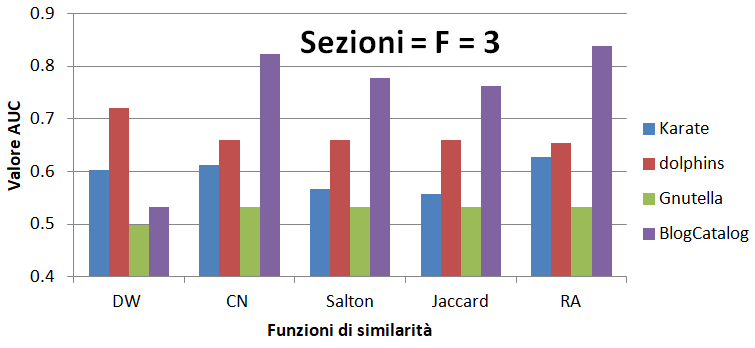
\includegraphics[width=\linewidth]{immagini/LP_fold3}
	\caption{\LPred\ con tre sezioni, $F=3$}
	\label{fig:LP_fold3}
\end{figure}
%
\begin{figure}[htp]
	\centering
	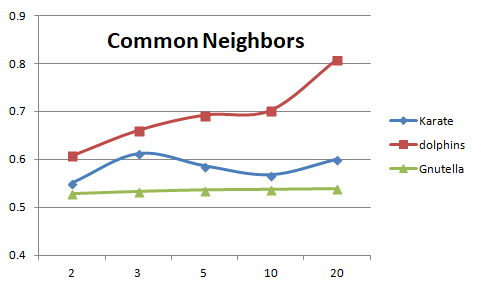
\includegraphics[width=\linewidth]{immagini/LP_CN}
	\caption{Andamento della metrica di Common Neighbors, su tre grafi distinti attraverso differenti percentuali di selezione (2-3-5-10-20)}
	\label{fig:LP_CN}
\end{figure}
%
\begin{figure}[htp]
	\centering
	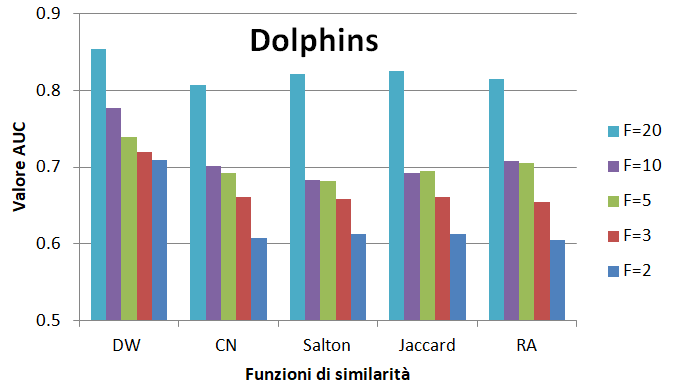
\includegraphics[width=\linewidth]{immagini/LP_Dolphins}
	\caption{Andamento del grafo dolphins, su diverse metriche, attraverso differenti percentuali di selezione}
	\label{fig:LP_Dolphins}
\end{figure}
%
Questo algoritmo ha tre possibili variabili su cui si può lavorare:
\begin{itemize}
	\item \textbf{Il parametro $F$} (dall'inglese fold) viene fissato nella Figura~\ref{fig:LP_fold3}. Si può notare come ogni grafo abbia un livello su cui si attesta; grazie al fatto che è estremamente denso, BlogCatalog ha un valore in media molto alto rispetto ai tre grafi restanti
	\item Nella Figura~\ref{fig:LP_CN} si lavora su un \textbf{unica metrica}. Si utilizza solo la funzione di similarità denominata Common Neighbors, che si basa sui nodi geometricamente vicini agli estremi di un arco all'interno del modello del grafo per valutare la somiglianza.\\
	Si può notare come all'aumentare del parametro $F$, il valore che si associa ad ogni grafo tende ad aumentare. Questo è dovuto ad un modello meglio addestrato perché dispone di più dati in partenza, e quindi si ha una migliore valutazione
	\item La Figura~\ref{fig:LP_Dolphins} è forse la più semplice da osservare in quanto è mostrato \textbf{un solo grafo}. Come prima si vede che l'influenza del parametro $F$ sul risultato finale è altissima. Si può notare che le prestazioni di DeepWalk sono leggermente più alte rispetto al resto che invece tende ad avere le stesse performance 
\end{itemize}
Si precisa che questi sono degli esempi rappresentativi dell'andamento generale, che però non viene riportato in quanto sarebbe molto complesso da comprendere.
%
\section{Classificazione dei nodi}
Il problema della classificazione dei nodi/vertici punta a riconoscere, partendo dalla rappresentazione di un elemento, a quale classe questo appartenga. Per definizione, un elemento può appartenere ad una ed una sola classe, è tuttavia possibile pensare a gruppi interni ad altri gruppi o a sovrapposizioni. Per esempio, data la classe A e la classe B si ha che, per come sono state definite, tutti gli elementi di A appartengono anche a B ($ A \subseteq B$), di conseguenza $ A \cap B = A$. Tuttavia questo vale per l'insiemistica, nei problemi di classificazione, fra A e B, non c'è nessuna relazione e conseguentemente si ha che $ A \cap B = \emptyset$.%esempio anche per intersezione???
%
\subsection{Dinamiche di funzionamento}
Il punto di partenza è costante, dato il grafo lo si visita per generare i cammini e con questi s'invoca l'algoritmo che genera il modello. Il modello viene disordinato e spezzato secondo il parametro di \textbf{training ratio $T_r$}, ossia la percentuale d'addestramento, questo indica la percentuale del modello che dovrà essere usata per l'addestramento, la restante sarà per i test.\\
In aggiunta si considerano anche le etichette o classi d'appartenenza, quindi per ogni nodo si ha una tripletta contenente:
\begin{itemize}
	\item ID del nodo che normalmente non viene considerato
	\item il vettore di numeri reali che lo rappresenta, vengono presi dal modello
	\item l'identificativo della classe a cui si appartiene
\end{itemize}
Con questi dati viene addestrata la \textbf{funzione di classificazione}, o \textbf{classificatore}, il cui scopo sarà predire la classe d'appartenenza dato in input il vettore rappresentativo di un nodo.\\
\\
In seguito per ogni nodo appartenente all'insieme di test si cerca di predire la sua classe sottoponendo il suo vettore al classificatore. Una volta terminato, si confronta se l'esito corrisponde con la reale classe, nota grazie allo stesso file di etichette utilizzato per l'addestramento.\\
È importante far notare che il modello viene spezzato in due perché il classificatore deve essere addestrato su dati diversi da quelli che prenderà in seguito in input. Se così non fosse non ci sarebbe nulla da predire in quanto i dati passati vengono ricordati e ed è impossibile sbagliare una risposta.\\
\\
La valutazione delle predizioni effettuate può avvenire mediante un metodo semplice ossia il \textbf{tasso d'errore}, che corrisponde alla Formula~\ref{eq:tasso_errore}. Si contano quanti errori si son fatti rispetto al totale o in alternativo si usa il metodo opposto ossia \textbf{l'accuratezza}, definita nella Formula~\ref{eq:accuratezza}, che conta i risultati con esito positivo rispetto al totale.
%
\begin{equation}
	T_{err} = \frac{N(errori)}{N(previsioni)}
	\label{eq:tasso_errore}
\end{equation}
%
\begin{equation}
	Acc = 1 - T_{err} = 1 - \left( \frac{N(errori)}{N(previsioni)} \right) = \frac{N(corretti)}{N(previsioni)}
	\label{eq:accuratezza}
\end{equation}
%
Se si vogliono fare delle misurazioni particolari si sfrutta invece la \textbf{matrice di confusione}, mostrata in Tabella~\ref{tab:matrice_confusione}, ideata inizialmente per valutare casi con solo due opzioni (Sì-positivo / No-negativo). Può essere generalizzata per gestire la valutazione di un classificatore con più di due esiti, tramite due approcci differenti.
\begin{itemize}
	\item si amplia la matrice per avere invece che due righe e due colonne, K righe e K colonne.\\
	Dove K è il numero di possibili valori ritornati dal classificatore
	\item si possono creare K matrici di confusione e ogni volta si sceglie una specifica classe come positiva, tutte le altre vengono implose nel valore negativo
\end{itemize}
%
\begin{multicols}{2}
\begin{center}
	\begin{tabular}{cc|c|c|}
		 &  & \multicolumn{2}{|c|}{Previsione}\\
		 &  & Sì & No\\
		 \hline
		 Risposta & Sì & TP & FN\\
		 \hline
		 corretta & No & FP & TN\\
		\hline
	\end{tabular}
	\captionof{table}{Viene rappresentata una matrice di confusione}
	\label{tab:matrice_confusione}
	%
	\begin{tabular}{|c|c|}
		\hline
		TP & True Positive \\
		FN & False Negative \\
		FP & False Positive \\
		TN & True Negative \\
		\hline
	\end{tabular}
	\label{tab:MC_significato}
	\captionof{table}{Significato delle sigle della matrice di confusione}
\end{center}
\end{multicols}
%
Da questa matrice possiamo estrarre diverse misurazioni:
\begin{itemize}
	\item \textbf{accuratezza} qui prende una nuova formulazione: $\displaystyle Acc = \frac{TP + TN}{TP + TN + FP + FN} $
	\item \textbf{sensibilità} penalizza le risposte negative sbagliate (FN), di conseguenza è meglio dare per positivo un esito se non è certo.\\
	Definita come: $\displaystyle S = \frac{TP}{TP + FN} $
	\item \textbf{precisione} penalizza le risposte positive sbagliate (FP), di conseguenza è meglio dare per negativo un esito se non è certo.\\
	Definita come: $\displaystyle P = \frac{TP}{TP + FP} $
	\item \textbf{Macro} precisione/sensibilità è la media aritmetica fra più valori di S o di P.\\
	Definita come: $\displaystyle Macro_{S} = \frac{S_1 + ... + S_n}{n} $
	\item \textbf{Micro} precisione/sensibilità è la media aritmetica delle componenti di S o di P prima di calcolarle, per poi considerarle un unica S o P.\\
	Definita come: $\displaystyle Micro_{P} = \frac{TP_1 + ... + TP_n }{ (TP_1 + ... + TP_n) + (FP_1 + ... + FP_n) } $
	\item \textbf{F1-Score} è la media armonica di: micro/macro/normale sensibilità e precisione.\\
	Definita come: $\displaystyle F1-Score = \frac{2}{ \frac{1}{S} + \frac{1}{P} } = \frac{2 \cdot S \cdot P}{ S + P }$
\end{itemize}
Nel caso mostrato, sensibilità e precisione non possono essere utilizzate in quanto ci sono troppi dati; mentre usare micro e macro non ha senso in quanto le classi sono perfettamente equivalenti, di conseguenza premiarne una a discapito di un'altra non ha significato. Per questo se serve si adotta l'F1-score. Tuttavia questa procedura non è veloce da calcolare, pertanto spesso si adotta il più semplice e veloce metodo dell'accuratezza.
%
\subsection{Esempio}
\begin{center}
	\begin{tabular}{|c|c|c|c|c|}
		\hline
		ID & x & Previsione & Classe & Corretta\\
		\hline
		$5$ & $9$ & $0$ & $1$ & $0$\\
		$1$ & $13$ & $0$ & $0$ & $1$\\
		$2$ & $15$ & $0$ & $0$ & $1$\\
		$3$ & $27$ & $0$ & $1$ & $0$\\
		$4$ & $34$ & $1$ & $1$ & $1$\\
		$8$ & $36$ & $1$ & $0$ & $0$\\
		$6$ & $48$ & $2$ & $2$ & $1$\\
		$7$ & $59$ & $2$ & $2$ & $1$\\
		\hline
	\end{tabular}
	\captionof{table}{Tabella riassuntiva del procedimento di classificazione dei vertici}
	\label{tab:dati_es_classify}
\end{center}
Tutti i dati dell'esempio sull'algoritmo di classificazione sono riassunti nella Tabella~\ref{tab:dati_es_classify}. Nella prima colonna abbiamo gli ID dei nodi coinvolti. La seconda colonna contiene il vettore rappresentativo di ogni nodo, qui per semplicità è stato ridotto ad un solo numero.
%
\begin{equation}
	C(x)=
		\begin{cases}
			\begin{array}{ll}
				0 & se \ x < 30\\
				1 & se \ 30 \leq x \ \&\  x < 45\\
				2 & se \ 45 \leq x
			\end{array}
		\end{cases}
	\label{eq:classificatore_esempio}
\end{equation}
%
Si assume il classificatore definito nella Formula~\ref{eq:classificatore_esempio}, che darà come risposte i valori contenuti nella colonna "Previsione".\\
Mentre nella colonna "Classe" è mostrato il valore autentico del nodo. Infine nell'ultima colonna è indicato se la previsione è risultata corretta o meno.\\
\\
Per una valutazione mediante accuratezza è sufficiente calcolare la media aritmetica dell'ultima colonna, ossia $ Acc = \frac{1+1+1+1+1}{8} = \frac{5}{8} = 0.625$. Mentre per l'F1-score sarebbe necessario calcolare sensibilità e precisione di ognuna delle 3 classi, riassumerli mediante micro o macro, ed infine arrivare ad un valore con F1-score.
%
\subsection{Applicazioni}
I grafi scelti per questa applicazione sono \cora\ (Figura~\ref{fig:VC_cora}) e \citeseer\ (Figura~\ref{fig:VC_citeseer}) perché fra quelli presentati nella Tabella~\ref{tab:dati_grafi} sono gli unici che sono forniti di attributi sui nodi. Questo permette di mostrare come l'utilizzo del grafo bipartito per l'introduzione degli attributi, modifica le prestazioni.
%
\begin{figure}[htp]
	\centering
	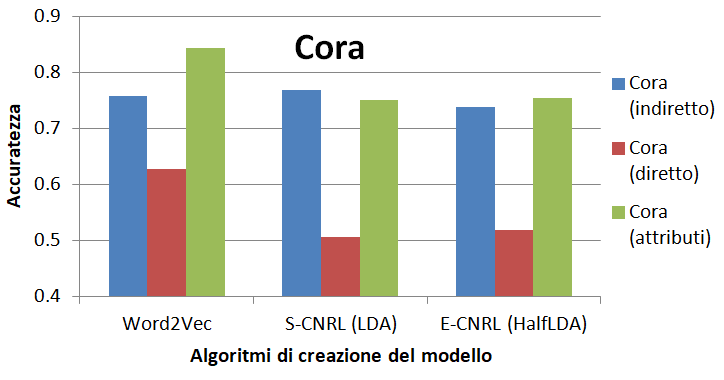
\includegraphics[width=\linewidth]{immagini/VC_cora}
	\caption{Andamento del grafo \cora, con 3 differenti algoritmi di creazione del modello e 3 diverse interpretazioni iniziali, valutato mediante l'accuratezza}
	\label{fig:VC_cora}
\end{figure}
%
\begin{figure}[htp]
	\centering
	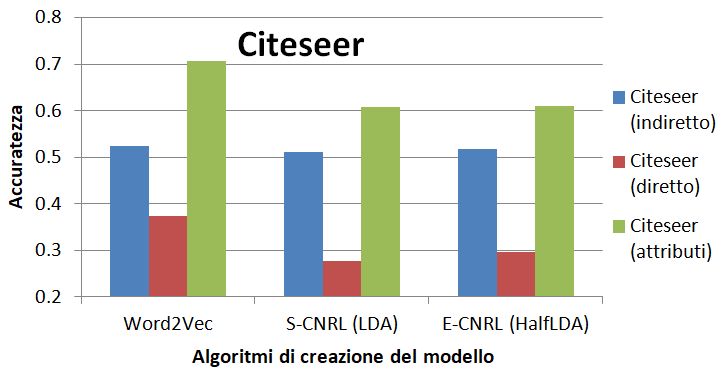
\includegraphics[width=\linewidth]{immagini/VC_citeseer}
	\caption{Andamento del grafo \citeseer, con 3 differenti algoritmi di creazione del modello e 3 diverse interpretazioni iniziali, valutato mediante l'accuratezza}
	\label{fig:VC_citeseer}
\end{figure}
%
Sull'asse delle ordinate vi sono i valori compresi nell'intervallo $[0, 1]$ misurati mediante la tecnica dell'accuratezza. Mentre sull'asse delle ascisse vi sono i tre algoritmi utilizzati per creare il modello del grafo partendo dai cammini. \wv\ è il metodo di controllo, mentre S-CNRL e E-CNRL che lavorano rispettivamente con LDA e HalfLDA, sono i nuovi algoritmi proposti. Entrambi per alcune parti continuano ad usare \wv.\\
Sia \cora\ che \citeseer\ sono grafi originariamente diretti (\textcolor{red}{misurazioni rosse}), tuttavia si è provato ad interpretarli anche come se fossero indiretti (\textcolor{blue}{campionamento blu}), l'ultimo andamento è dato dall'introduzione degli attributi (\textcolor{green}{dati verdi}).\\
Ecco alcuni dettagli che emergono dai due grafici:
\begin{itemize}
	\item \wv\ mostra prestazioni, anche se di poco, maggiori delle due alternative che invece tendono ad equivalersi
	\item la media dei valori delle misurazione nel grafico di \cora\ (Figura~\ref{fig:VC_cora}) è $0.696$ rispetto a quella di \citeseer\ (Figura~\ref{fig:VC_citeseer}) che è $0.491$, la prima risulta essere maggiore di circa $ \frac{2}{10}$ questo è dovuto anche al fatto che \cora\ abbia una $ densita' = \frac{archi}{nodi}$ maggiore rispetto a \citeseer
	\item un alta densità degli archi permette di creare molte interazioni fra i nodi e quindi il modello meglio rappresenta il grafo. Si noti però che questo non è sempre facile da individuare, qui è presente uno stacco evidente in quanto entrambi i grafi hanno un estremamente bassa densità si dice infatti che sono sparsi
	\item si è provato ad aumentare la densità, considerando ambo i grafi come indiretti (ogni arco indiretto può essere rappresentato come due archi diretti). Si ha quindi poco meno di un raddoppio della densità, è infatti possibile che un arco avesse già il suo opposto e quindi non risenta del cambiamento.\\
	L'effetto per entrambi è stato un innalzamento del valore medio lungo i 3 algoritmi usati
	\item con il grafo indiretto l'incremento di S-CNRL e E-CNRL è maggiore rispetto a quello di \wv . Questo può indicare, che \wv\ lavora molto bene con i grafi orientati a dispetto degli altri due metodi
	\item l'introduzione degli attributi tramite il grafo bipartito cambia notevolmente la situazione portando ad un incremento di prestazioni. Questi valori vanno confrontati con i dati del grafo orientato in quanto quello è il valore corretto. I punti blu del grafo non-orientato non sono comparabili in quanto servono a mostrare come la densità influisce sul risultato, rappresentano un nuovo grafo diverso dall'originale, e quindi non paragonabile
\end{itemize}
%
\section{Valutazione dell'individuazione di comunità}
Questa sezione ripercorre la parte principale del tirocinio, ossia l'integrazione degli attributi e la valutazione di un partizione mediante la modularità. Vengono presentate quattro situazioni ognuna approfondisce un aspetto affrontato.
%
\subsection{Confronto numero comunità}%1
%
\begin{figure}[htp]
	\centering
	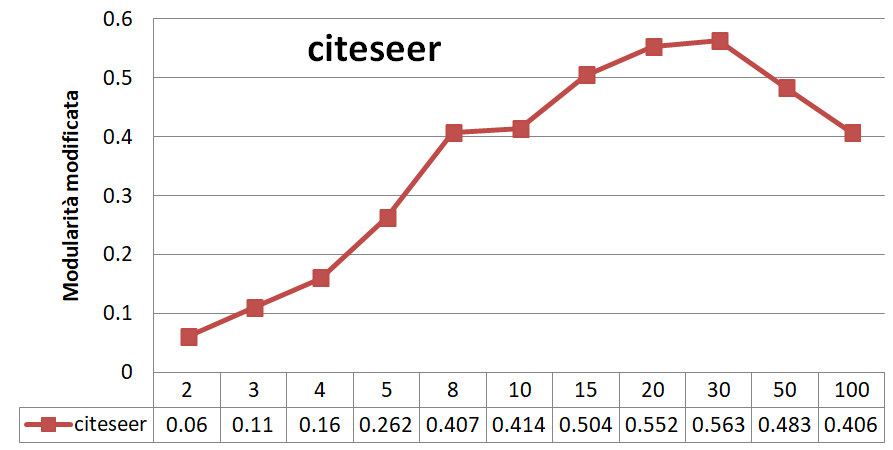
\includegraphics[width=\linewidth]{immagini/MOD_1_num_cmty}
	\caption{Accuratezza rappresentativa al variare del numero delle comunità da generare (2-3-4-5-8-10-15-20-30-50-100)}
	\label{fig:MOD_1_num_cmty}
\end{figure}
%
In Figura~\ref{fig:MOD_1_num_cmty} è possibile vedere l'andamento dell'algoritmo d'individuazione delle comunità LDA, applicato al grafo \citeseer\ di cui si considera solo la struttura, la valutazione vien fatta con la \mmod.\\
L'unico parametro che viene modificato è mostrato sull'asse delle ascisse ed è il numero di comunità che si vanno a ricercare all'interno del grafo. Ecco cosa s'osserva:
\begin{itemize}
	\item la progressione del numero di comunità da ricercare è stata scelta per mostrare la rapida crescita della modularità quando piccoli numeri sono coinvolti
	\item il valore calcolato su $2$ comunità è estremamente basso, perché difficilmente riesce a rappresentare a dovere una vasta selezione di nodi
	\item la modularità cresce con l'aumentare delle comunità, che premiano sempre più le peculiarità del grafo
	\item c'è un massimo compreso fra $30$ e $50$ dove questa crescita s'interrompe
	\item gli ultimi due dati $50$ e $100$ decrescono, questo è noto come il \textbf{problema dell'overfitting}, a causa di un addestramento eccessivo, il risultato raggiunto non è più in linea con le aspettative.\\
	Via via che i gruppi di nodi si stringono perdono di rappresentazione portando così ad un decremento della modularità. Si osserva questo fenomeno anche in Figura~\ref{fig:MOD_3_elaborazione}
\end{itemize}

\subsection{Metriche di valutazione}%2
Nella Tabella~\ref{tab:2_metriche} vengono mostrati i due grafi di \cora\ e \citeseer, valutati mediante tre differenti metriche di calcolo della modularità.\\
Ambo i grafi sono stati caricati senza considerare gli attributi dei nodi, ma solo la loro struttura. La creazione del modello è avvenuta con S-CNRL e il suo algoritmo LDA, tramite il quale sono state ricavate le $10$ comunità che vengono  valutate in Tabella.\\
Non ha senso confrontare i tre differenti metodi di calcolo della modularità, in quanto premiano aspetti differenti. Inoltre ognuno si posiziona su un diverso ordine di grandezza.Spicca sopratutto \mover\ che presenta tutti i valori molto vicini a 0, questo perché, come riporta la Tabella~\ref{tab:dati_grafi}, ambo i grafi sono estremamente sparsi e, a causa di ciò, \mover\ ha il valore assoluto della modularità calcolata vicino a $0$.\\
Tutti i metodi assegnano a \cora\ il valore più alto, e questo fa capire che, se una partizione è nettamente migliore di un'altra, allora verrà premiata indipendentemente dalla metrica di valutazione usata.\\
La \mmod\ è stata scelta come metrica ufficiale degli esperimenti, non solo per il fatto che è quella usata nell'articolo di \cnrl, ma anche perché presenta dei valori facilmente analizzabili e comprensibili. \mover\ funziona bene ma è sempre difficile comprendere i risultati a cui s'arriva rischiando incomprensioni.
%
\begin{center}
	% Schema num: 2 -> confronto metriche (cmty=10, no_att, valutazione con grafo norm, metric 8 -> HalfLDA)
	\begin{tabular}{|l|c|c|c|} % \multicolumn{2}{|c|}{testo}  \multirow{2}{*}{testo}   $ \e{-}$
		\hline
		\ & \mmax & \mover & \mmod \\
		\hline
		\cora & $2.04$ \e{-1} & $1.21$ \e{-5} & $5.31$ \e{-1} \\
		\citeseer & $8.42$ \e{-2} & $-3.55$ \e{-6} & $3.67$ \e{-1} \\
		%2.04E-01	1.21E-05	5.31E-01
		%8.42E-02	-3.55E-06	3.67E-01
		\hline
	\end{tabular}
	\captionof{table}{Confronto fra i metodi di modularità spiegati, partendo dal grafo normale con $10$ comunità}
	\label{tab:2_metriche}
\end{center}

%\begin{center}
%	\begin{tabular}{|l|c|c|} % \multicolumn{2}{|c|}{testo}  \multirow{2}{*}{testo}   $ \e{-}$
%		\hline
%		\ & \cora & \citeseer \\
%		\hline
%		\mmax & $2.04$ \e{-1} & $8.42$ \e{-2} \\  
%		\mover & $1.21$ \e{-5} & $-3.55$ \e{-6} \\  
%		\mmod & $5.31$ \e{-1} & $3.67$ \e{-1} \\  
%		\hline
%	\end{tabular}
%	\captionof{table}{Confronto fra i metodi di modularità spiegati, partendo dal grafo normale con $10$ comunità}
%	\label{tab:2_metriche}
%\end{center}

%
\subsection{Confronto metodi d'elaborazione}%3
%
\begin{figure}[htp]
	\centering
	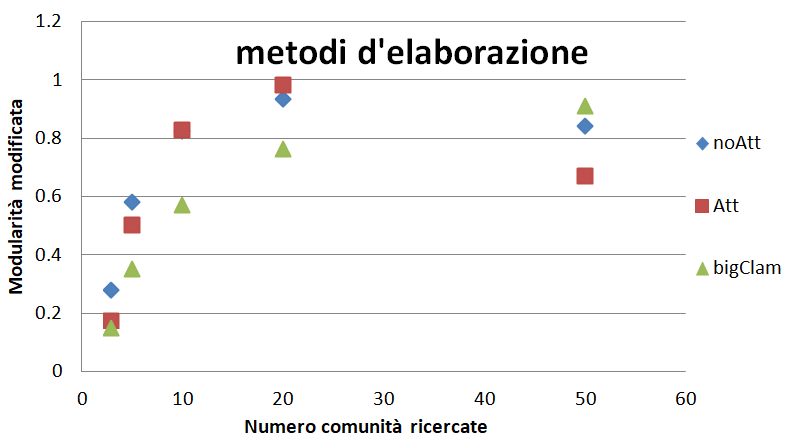
\includegraphics[width=\linewidth]{immagini/MOD_3_elaborazione}
	\caption{Prestazioni dei diversi procedimenti d'elaborazione del modello sul grafo \cora, al variare del numero di comunità da ricercare (3-5-10-20-50)}
	\label{fig:MOD_3_elaborazione}
\end{figure}
%
In Figura~\ref{fig:MOD_3_elaborazione} vengono confrontati tre differenti metodi d'elaborazione dei grafi, il cui scopo è trovare le comunità.\\
Viene presentato il grafo \cora\ su cui si è applicata una progressione da $3$ a $50$ comunità, valutate tramite la \mmod. \\
I tre metodi utilizzati sono:
\begin{itemize}
	\item \textbf{noAtt}: si considera in partenza unicamente la struttura del grafo, dai cui si ricavano i cammini e vengono elaborati con LDA
	\item \textbf{Att}: oltre ai cammini derivanti dalla struttura si crea anche il grafo bipartito degli attributi, il tutto elaborato sempre mediante LDA
	\item \textbf{bigClam}: è il metodo tratto dall'articolo "Overlapping community detection at scale: a nonnegative matrix factorization approach"\cite{bigClam_paper}, implementato dall'università di Stanford\cite{bigClam_code}.\\
	È stato scelto come algoritmo di controllo per verificare l'andamento delle prestazioni di S-CNRL
\end{itemize}
Dalla figura possiamo capire:
\begin{itemize}
	\item come per Figura~\ref{fig:MOD_1_num_cmty}, con l'aumentare del numero di comunità si ha il problema dell'overfitting.\\
	Per \citeseer\ il problema si rivela quando si cercano $50$ comunità e così è per \cora, questo sembra non valere per bigClam anche se è inevitabile che accada con numeri molto alti di comunità da individuare
	\item durante la crescita le prestazioni di bigClam restano costantemente inferiori
	\item l'apice è raggiunto mediante gli attributi con $20$ comunità ad un valore di $Q=0.986$. È importante notare che non tutti gli apici dei vari metodi si posizionano a $20$ comunità. Al contrario, BigClam sembra aver questo massimo oltre le $50$ comunità
	\item valutare il grafo mediante e senza gli attributi sembra non influire troppo, anche se così non dovrebbe essere (caso meglio analizzato in Tabella~\ref{tab:4_valutazioni})
\end{itemize}
%
\subsection{Confronto criteri di valutazione}%4
%
\begin{center}
	% Schema num: 4 -> confronto valutazioni
	\begin{tabular}{|cc|c|c|} % \multicolumn{2}{|c|}{testo}  \multirow{2}{*}{testo}   $ \e{-}$
		\hline
		\multicolumn{2}{|c|}{\textbf{\cora}} & \multicolumn{2}{|c|}{valutazione} \\
		\multicolumn{2}{|c|}{\ } & struttura & ipergrafo \\
		\hline
		\multirow{2}{*}{elaborazione} & noAtt & $8.24$ \e{-1} & $9.83$ \e{-3} \\
		& Att & $8.29$ \e{-1} & $2.33$ \e{-2} \\
		\hline
		\hline
		\hline
		\multicolumn{2}{|c|}{\textbf{\citeseer}} & \multicolumn{2}{|c|}{valutazione} \\
		\multicolumn{2}{|c|}{\ } & struttura & ipergrafo \\
		\hline
		\multirow{2}{*}{elaborazione} & noAtt & $4.14$ \e{-1} & $8.86$ \e{-6} \\
		& Att & $4.14$ \e{-1} & $2.30$ \e{-2} \\
		\hline
	\end{tabular}
	\captionof{table}{Misurazione delle comunità, generate attraverso due differenti metodi d'elaborazione, analizzate su due tipologie di valutazione}
	\label{tab:4_valutazioni}
\end{center}
Nella Tabella~\ref{tab:4_valutazioni} vengono mostrati entrambi i grafi di \cora\ e \citeseer, su ognuno son state fatte quattro differenti valutazioni.\\
Sulle righe vi sono i metodi  d'elaborazione utilizzati per trovare le comunità:
\begin{itemize}
	\item \textbf{noAtt} indica che del grafo è stata utilizzata solamente la struttura per la generazione dei cammini
	\item \textbf{Att} indica invece che oltre ai dati della struttura vengono utilizzati anche gli attributi introdotti tramite il grafo bipartito
\end{itemize}
%
Sulle colonne sono invece riportati i due metodi per la valutazione della partizione generata:
\begin{itemize}
	\item \textbf{struttura} indica che il grafo utilizzato per la valutazione, tramite \mmod, è quello originale, che contiene solo la struttura
	\item \textbf{ipergrafo} il grafo per la valutazione con \mmod\ contiene anche gli archi degli attributi, non è possibile utilizzare un grafo bipartito in quanto contiene nodi (l'insieme N2) non appartenenti al grafo originario, si opta quindi per l'ipergrafo.\\
	Quello qui utilizzato, rispetto a quello mostrato in Figura~\ref{fig:7transform_hyper}, mantiene anche gli archi originali e per non creare incoerenze considera tutti gli archi come diretti, ciò porta a più d'un raddoppio del numero d'archi, partendo da un numero base già elevatissimo
\end{itemize}
%
Dalla Figura~\ref{fig:MOD_3_elaborazione} si può vedere che con $10$ comunità la valutazione di \cora, elaborato con e senza attributi, è molto simile. Si è scelto d'utilizzare le $10$ comunità per osservare le variazioni quando si adotta una valutazione attraverso l'ipergrafo.\\
Ecco cosa si può notare:
\begin{itemize}
	\item per la scelta del numero di comunità i dati di \cora, valutati sulla struttura, sono pressoché uguali
	\item per \citeseer\ accade lo stesso, qui i due valori sono identici.\\
	Il dato di $4.14$ \e{-1} è già apparso in Tabella~\ref{fig:MOD_1_num_cmty}
	\item se la valutazione avviene sull'ipergrafo sia nel caso di \cora\ che di \citeseer\ il valore più alto viene generato con l'elaborazione effettuata sugli attributi.\\
	È in linea con le aspettative, perché i cammini aggiunti dal grafo bipartito vanno a descrivere una sezione che l'elaborazione, utilizzante solo la struttura, non può conoscere e quindi non vi si può adattare
	\item tutte le valutazioni sull'ipergrafo sono così vicine allo $0$ perché l'Espressione~\ref{eq:d_in-out}, parte della Formula~\ref{eq:m_mod}, della \mmod, in presenza di un grafo molto denso, ed è questo il caso, abbassa notevolmente il valore della misurazione
\end{itemize}
%
Nonostante i dati mostrati in Tabella~\ref{tab:4_valutazioni} siano perfettamente in linea con le aspettative, non è possibile affermare che quanto mostrato in questa sottosezione sia sempre vero in ogni possibile situazione, in quanto i risultati restituiti dalla \mmod\ presentano una non trascurabile variabilità.



\chapter{Conclusioni}\label{chap:4}
Seguono alcune considerazioni personali sul lavoro affrontato e su come è stato svolto.
\section*{Conclusioni tecniche}
Vorrei evidenziare le potenzialità dell'uso degli attributi nella creazione dei modelli.\\
Durante il tirocinio sono stati indagati solo alcuni dei metodi esistenti per l'introduzione di questi dati aggiuntivi. Ne esistono molti altri, ognuno con i suoi vantaggi e svantaggi. Non so se gli approcci da noi utilizzati sono i migliori o quelli con più potenzialità, ma comunque abbiamo riscontrato che lavorano bene e hanno portato ad un miglioramento.\\
Uno dei vantaggi principali è che, basandosi su delle meccaniche semplici, è potenzialmente fattibile integrarli con altri metodi, portando ad ulteriori miglioramenti. Uno svantaggio evidente è il tempo d'esecuzione. Il codice iniziale di \cnrl\ è molto veloce, l'introduzione delle meccaniche proposte in questa tesi hanno appesantito molto il costo computazionale. Questo è ancor più evidente quando, come nel nostro caso, si lavora con grafi estremamente sparsi che però dispongono di molti attributi.\\
Probabilmente questo approccio dovrà essere ancora e ancora sviluppato, ma non è escluso che potrà dare un suo valido contributo.
%
\section*{Conclusioni personali}
Affacciarsi per la prima volta a questo campo è molto complesso.\\
È possibile, anche se estremamente difficoltoso, comprendere tutte le meccaniche degli algoritmi che si vanno ad utilizzare. Essendo un progetto molto vasto personalmente ho preferito appoggiarmi a svariate parti di codice già ideate, scritte e testate.\\
I dataset su cui si va ad operare sono troppo ampi e questo comporta che non se ne possa tener traccia. Gli errori sono complicati da individuare poiché non è possibile eseguire manualmente le operazioni svolte dal codice, nonostante si conoscano nel dettaglio come lavorano gli algoritmi. È fondamentale non sottovalutare la mole del progetto su cui si lavora e non tralasciare nessun dettaglio finché è ancora possibile individuarlo, testarlo e correggerlo.\\
La complessità maggiore che personalmente ho incontrato sta nel settaggio dei parametri.\\
Visto la moltitudine di possibilità di cui si dispone, risulta complesso abbracciarle tutte, per comprendere come impostare i parametri che regolano la gestione dei dati all'interno del codice. Spesso alcuni settaggi sono disponibili solo in alcune situazioni o dipendono da delle impostazioni. Un esecuzione avvenuta con parametri errati non rispecchia le aspettative, e porta a dover rivedere il tutto.\\
In conclusione, le tante sfaccettature di questo argomento lo rendono complesso e difficile, è quindi necessario prestare sempre estrema attenzione al metodo di lavoro.

%\end{document}




